\documentclass[12pt,a4paper]{article}

\usepackage{ctex}
\usepackage{graphicx}
\usepackage{booktabs}
\usepackage{amsmath}
\usepackage{csvsimple}
\usepackage{hyperref}
\usepackage{float}

\begin{document}

\begin{center}
    {\LARGE\bfseries NewtonRings Experiment Report}

    \vspace{0.5em}

    Zheng Zhihao
\end{center}

\vspace{0.5em}

\noindent
\begin{minipage}[t]{0.48\textwidth}
    \centering
    \textbf{Newton's Rings Experimental Data}

    \vspace{0.5em}
    \resizebox{\textwidth}{!}{%
        \begin{tabular}{|c|c|c|c|c|}
            \hline
            $k$
            & $x_k\, (\mathrm{mm})$
            & $x'_k\, (\mathrm{mm})$
            & $r_k\, (\mathrm{mm})$
            & $r_k^2\, (\mathrm{mm}^2)$ \\
            \hline
            \csvreader[
                head to column names
            ]{Origin-Data.csv}{
               1=\K,
               2=\XK,
               3=\XPK,
               4=\RK,
               5=\RKtwo,
               }{
                \K & \XK & \XPK & \RK & \RKtwo \\
                \hline
               }
        \end{tabular}%
    }
\end{minipage}
\hfill
\begin{minipage}[t]{0.48\textwidth}
    \centering

    \textbf{Linear Fit}

    \vspace{0.5em}

    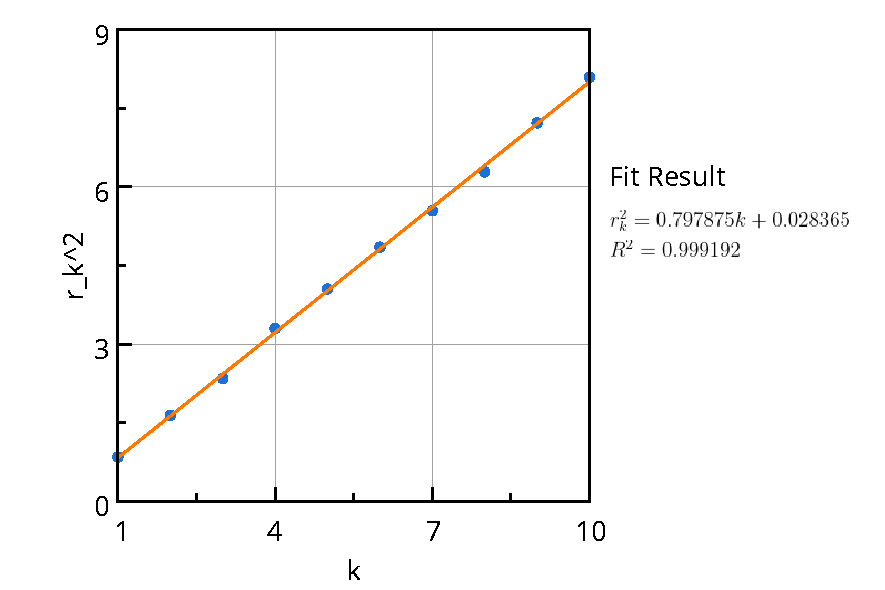
\includegraphics[width=\textwidth]{plot.pdf}

    \vspace{0.5em}

    Linear fit of $r_k^2$ versus $k$
\end{minipage}

\[
R=\frac{\alpha}{\lambda_{\mathrm{Na}}}
=\frac{0.797875\ \mathrm{mm}^2}
{5.893\times10^{-4}\ \mathrm{mm}}
=1.354\times10^3\ \mathrm{mm}
=1.354\ \mathrm{m}
\]

\noindent
\begin{minipage}[t]{0.48\textwidth}
    \centering
    \textbf{LED Experimental Data}

    \vspace{0.5em}
    \resizebox{\textwidth}{!}{%
        \begin{tabular}{|c|c|c|c|c|}
            \hline
            $k$
            & $x_k\, (\mathrm{mm})$
            & $x'_k\, (\mathrm{mm})$
            & $r_k\, (\mathrm{mm})$
            & $r_k^2\, (\mathrm{mm}^2)$ \\
            \hline
            \csvreader[
                head to column names
            ]{Origin-Data2.csv}{
               1=\K,
               2=\XK,
               3=\XPK,
               4=\RK,
               5=\RKtwo,
               }{
                \K & \XK & \XPK & \RK & \RKtwo \\
                \hline
               }
        \end{tabular}%
    }
\end{minipage}
\hfill
\begin{minipage}[t]{0.48\textwidth}
    \centering

    \textbf{Linear Fit}

    \vspace{0.5em}

    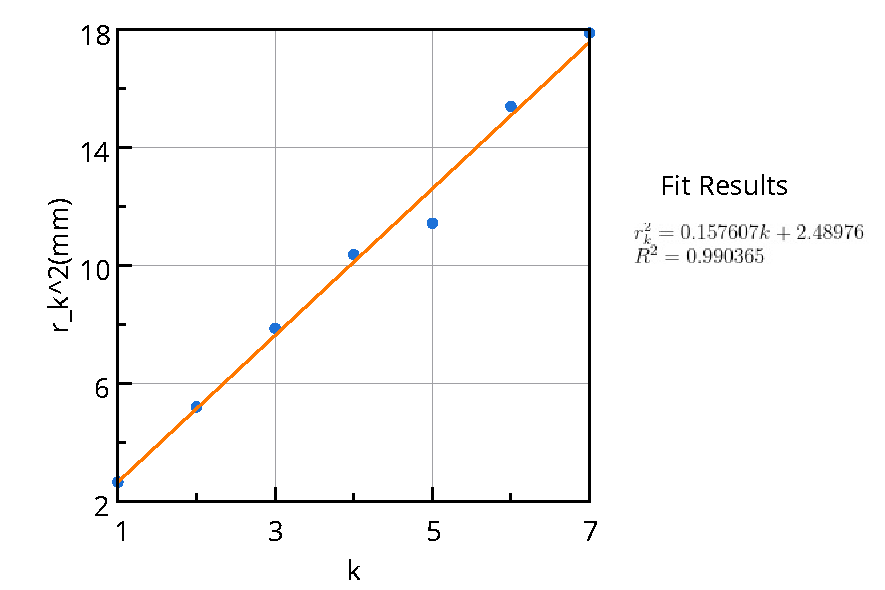
\includegraphics[width=\textwidth]{plot2.pdf}

    \vspace{0.5em}

    Linear fit of $r_k^2$ versus $k$
\end{minipage}

\[
\lambda_{\mathrm{LED}}
=\frac{\tilde{\alpha}}{\alpha}\lambda_{\mathrm{Na}}
=468.3\ \mathrm{nm}
\]

\noindent
Detailed data and figures are available at:\\
\url{https://github.com/alizeisnotalice/physics-experiment/NewtonRings}

\end{document}
